\documentclass[svgnames]{beamer}

\usepackage[utf8]{inputenc}
\usepackage[T1]{fontenc}
\usepackage{tgadventor}
\usepackage{microtype}

\setbeamertemplate{headline}{}
\setbeamertemplate{navigation symbols}{}
\setbeamertemplate{footline}{}

\usepackage{tikz}
\usetikzlibrary{calc}
\usetikzlibrary{positioning}
\usetikzlibrary{decorations.pathmorphing, decorations.pathreplacing}
\usetikzlibrary{matrix}
\usetikzlibrary{arrows}

\definecolor{kernel}         {named} {red}
\definecolor{scheduler init} {named} {PaleVioletRed}
\definecolor{yield}          {named} {violet}
\definecolor{add 1}          {named} {Green}
\definecolor{mul 2}          {named} {MediumBlue}

\tikzset{ every picture/.style = { ultra thick}
        , process/.style            = {color=white, draw=#1, fill=#1, rounded corners}
        , can jump to/.style        = {color=#1,                                                                  ->}
        , can store to/.style       = {color=#1, decorate, decoration={snake, pre length = 1mm, post length=1mm}, ->}
        , needs jump access/.style  = {can jump to=#1,  dashed}
        , needs store access/.style = {can store to=#1, dashed} }

\begin{document}
\begin{frame}
\begin{center}
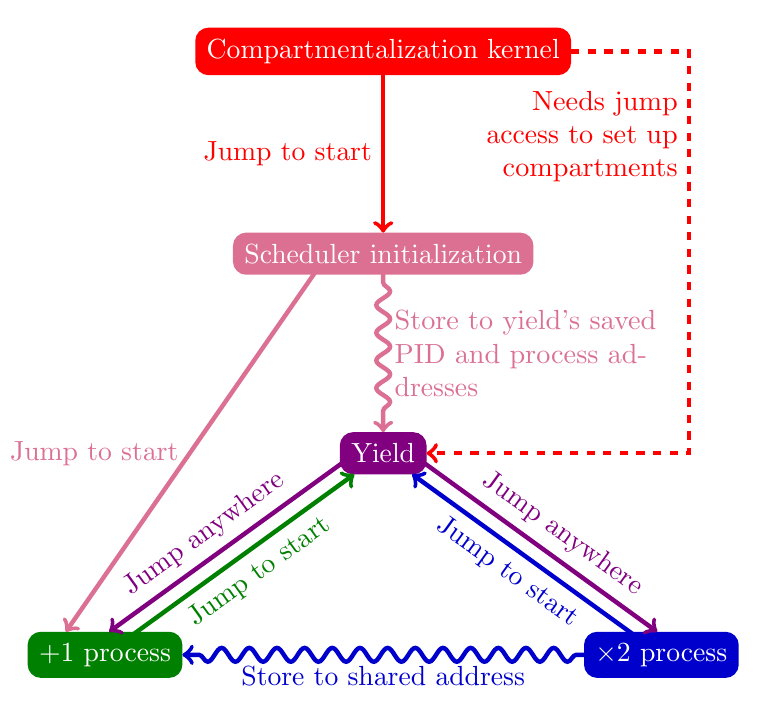
\begin{tikzpicture}[node distance=2cm]
  \node (kernel)         [process = kernel]                                                      {Compartmentalization kernel} ;
  \node (scheduler init) [process = scheduler init, below       =             of kernel]         {Scheduler initialization} ;
  \node (yield)          [process = yield,          below       =             of scheduler init] {Yield} ;
  \node (add 1)          [process = add 1,          below left  = 2cm and 2cm of yield]          {$+1$ process} ;
  \node (mul 2)          [process = mul 2,          below right = 2cm and 2cm of yield]          {$\times 2$ process} ;
  
  \path[shorten < = -1mm]
    (kernel)            edge[can jump to = kernel]
                        node[left]
                          {Jump to start}
      (scheduler init)
    (kernel.east)       edge[needs jump access = kernel, shorten < = 0cm, to path = {-- ++(1.5cm,0) |- (\tikztotarget) \tikztonodes}]
                        node[above left = 3.3cm and 0cm, align = right, text width = 3.1cm]
                          {Needs jump \mbox{access} to set up compartments}
      (yield.east)
    (scheduler init)    edge[can store to = scheduler init]
                        node[right, text width=3.4cm]
                          {Store to yield's saved PID and process addresses}
      (yield)
    (scheduler init)    edge[can jump to = scheduler init, transform canvas={xshift=-.7cm}]
                        node[left]
                          {Jump to start}
      (add 1)
    (yield)             edge[can jump to = yield, shorten < = -.25cm, transform canvas={xshift=-.35cm}]
                        node[above,sloped]
                          {Jump anywhere}
      (add 1)
    (yield)             edge[can jump to = yield, shorten < = -.25cm, transform canvas={xshift=+.35cm}]
                        node[above,sloped]
                          {Jump anywhere}
      (mul 2)
    (add 1)             edge[can jump to = add 1]
                        node[below,sloped]
                          {Jump to start}
      (yield)
    (mul 2)             edge[can jump to = mul 2]
                        node[below,sloped]
                          {Jump to start}
      (yield)
    (mul 2)             edge[can store to = mul 2]
                        node[below]
                          {Store to shared address}
      (add 1) ;
\end{tikzpicture}
\end{center}
\end{frame}

\begin{frame}
\begin{center}
\footnotesize
\begin{tikzpicture}
  \newlength\MemRegionHeight
  \setlength\MemRegionHeight{.9cm}
  \matrix[ matrix of nodes, every node/.style={draw=black}, color=white
         , row sep=-1.6pt, minimum width=8cm, minimum height=\MemRegionHeight
         , one address/.style={minimum height=\MemRegionHeight/2} ]
  {
    |[fill=kernel]             (kernel code)|       Compartmentalization kernel code \\
    |[fill=kernel]             (kernel data)|       Compartmentalization kernel service arguments \\
    %
    |[fill=scheduler init]     (init code)|         Scheduler initialization code \\
    %
    |[fill=yield]              (yield code)|        Yield code \\
    |[fill=yield, one address] (yield pid)|         Scheduled PID \\
    |[fill=yield, one address] (yield proc 1 pc)|   Process 1's stored pc \\
    |[fill=yield]              (yield proc 1 regs)| Process 1's stored registers \\
    |[fill=yield, one address] (yield proc 2 pc)|   Process 2's stored pc \\
    |[fill=yield]              (yield proc 2 regs)| Process 2's stored registers \\
    %
    |[fill=add 1]              (add 1 code)|        $+1$ process code \\
    |[fill=add 1, one address] (shared data)|       Shared user data \\
    %
    |[fill=mul 2]              (mul 2 code)|        $\times2$ process code \\
  } ;
  
  \foreach \mems/\color in { {kernel code}/kernel%
                           , {yield code, yield pid, yield proc 1 pc, yield proc 1 regs, yield proc 2 pc}/yield%
                           , {add 1 code}/add 1}
  {
    \foreach \mem in \mems {
      \message{\mem}
      \draw[draw=\color, dashed, line width=3.2pt, shorten < = 3pt, shorten > = 3pt]
        ($(\mem.south west)+(0,.8pt)$) -- ($(\mem.south east)+(0,.8pt)$) ;
    }
  }
  
  \useasboundingbox (current bounding box.north west) rectangle (current bounding box.south east) ;
  
  \draw[color=add 1, decorate, decoration={brace, amplitude=.15cm}]
    ($(shared data.south west)+(-.1cm,3.2pt)$) -- ($(add 1 code.north west)+(-.1cm,-3.2pt)$)
    coordinate[midway, xshift=-.25cm] (add 1 all) ;
  \draw[color=mul 2, decorate, decoration={brace, amplitude=.15cm}]
    ($(mul 2 code.south west)+(-.1cm,3.2pt)$) -- ($(mul 2 code.north west)+(-.1cm,-3.2pt)$)
    coordinate[midway, xshift=-.25cm] (mul 2 all) ;
  
  \path[can store to/.style={color=########1, -latex}]
    (kernel code.west) edge[can jump to=kernel,          out=180, in=180]            ($(init code.north west)+(0,-2.4pt)$)
                       edge[can jump to=kernel, dashed,  out=180, in=180]            ($(yield code.north west)+(0,-2.4pt)$)
    (init code.west)   edge[can jump to=scheduler init,  out=180, in=180]            ($(add 1 code.north west)+(0,-2.4pt)$)
                       edge[can store to=scheduler init, out=180, in=180]            (yield pid.west)
                       edge[can store to=scheduler init, out=180, in=180]            (yield proc 1 pc.west)
                       edge[can store to=scheduler init, out=180, in=180]            (yield proc 2 pc.west)
    (yield code.west)  edge[can jump to=yield,           out=180, in=180]            (add 1 all)
                       edge[can jump to=yield,           out=180, in=180]            (mul 2 all)
    (mul 2 code.east)  edge[can jump to=mul 2,           out=0,   in=+30]            ($(yield code.north east)+(0,-3.0pt)$)
    (add 1 code.east)  edge[can jump to=add 1,           out=0,   in=-30]            ($(yield code.north east)+(0,-6.0pt)$)
    (mul 2 code.east)  edge[can store to=mul 2,          out=0,   in=0, looseness=3] (shared data.east)
    ;
\end{tikzpicture}
\end{center}
\end{frame}
\end{document}
